\usepackage{pgfpages}
\usepackage{graphicx}
\usepackage{ucs}
\usepackage[utf8x]{inputenc}
\usepackage{tabularx}

\usepackage{polski}

\mode<presentation>
{
    \usetheme{CambridgeUS}
}

\title[Modernizacja oprogramowania CICTS]{Modernizacja oprogramowania. \\ Studium przypadku CICTS.\\\textsl{\small Założenia i zakres pracy.}}
\author[A. Trojnar]{Adam Trojnar}
\institute[WSKSiM, INF3]{Wyższa Szkoła Kultury Społecznej i Medialnej w Toruniu}
\date{2012.04.25}

\setbeamercovered{transparent=35}

\begin{document}

\begin{frame}
  \titlepage
\end{frame}

\begin{frame}{Plan wystąpienia}
	\tableofcontents

	Długość: $<$10 minut
\end{frame}

\section{Układ pracy}

\subsection{Streszczenie części teoretycznej}

\begin{frame}{Ramowy plan pracy dyplomowej}{(Opiekun naukowy: dr Tomasz Kowalski)}
    \begin{enumerate}
    \item Wstęp
    \item Wybrane aspekty modernizacji oprogramowania
        \uncover<2->{
            \begin{enumerate}
            \item<alert@2> Motywacje dla podejmowania modernizacji

%% wpisać hasła lub literaturę tak jak poniżej 

            \item<alert@3> Strategie modernizacji

\only<3>{\footnotesize
    WMU (Sahin i Zahedi, 2001), 
    SABA (Bennett i inni, 1999), 
    Renaissance (Warren i Ransom, 2002), itd.
}

            \item<alert@4> Zarządzanie ryzykiem
%% wpisać hasła lub literaturę tak jak powyżej
            \item<alert@5> Wyzwania techniczne i organizacyjne
%% wpisać hasła lub literaturę tak jak powyżej
            \item<alert@6> Opcje modernizacji
%% wpisać hasła lub literaturę tak jak powyżej
            \end{enumerate}
        }
    \item Koordynowanie wydarzeń przez CICTS
        \uncover<7->{
            \begin{enumerate}
            \item Opis ideowy
            \item Analiza istniejącego oprogramowania wspierającego
            \item \textsf{org.cicts.Scheduler} -- oprogramowanie zmodernizowane
                \begin{enumerate}
                \item Specyfikacja wymagań niefunkcjonalnych
                \item Wybrane zagadnienia implementacyjne
                \end{enumerate}
            \end{enumerate}
        }
    \item Podsumowanie
    \end{enumerate}
\end{frame}

\section[Studium przypadku CICTS]{Studium przypadku CICTS. (Część praktyczna).}

\subsection{Istniejąca aplikacja}

\begin{frame}{Aktualna aplikacja CICTS}{tutuł obrazka}
   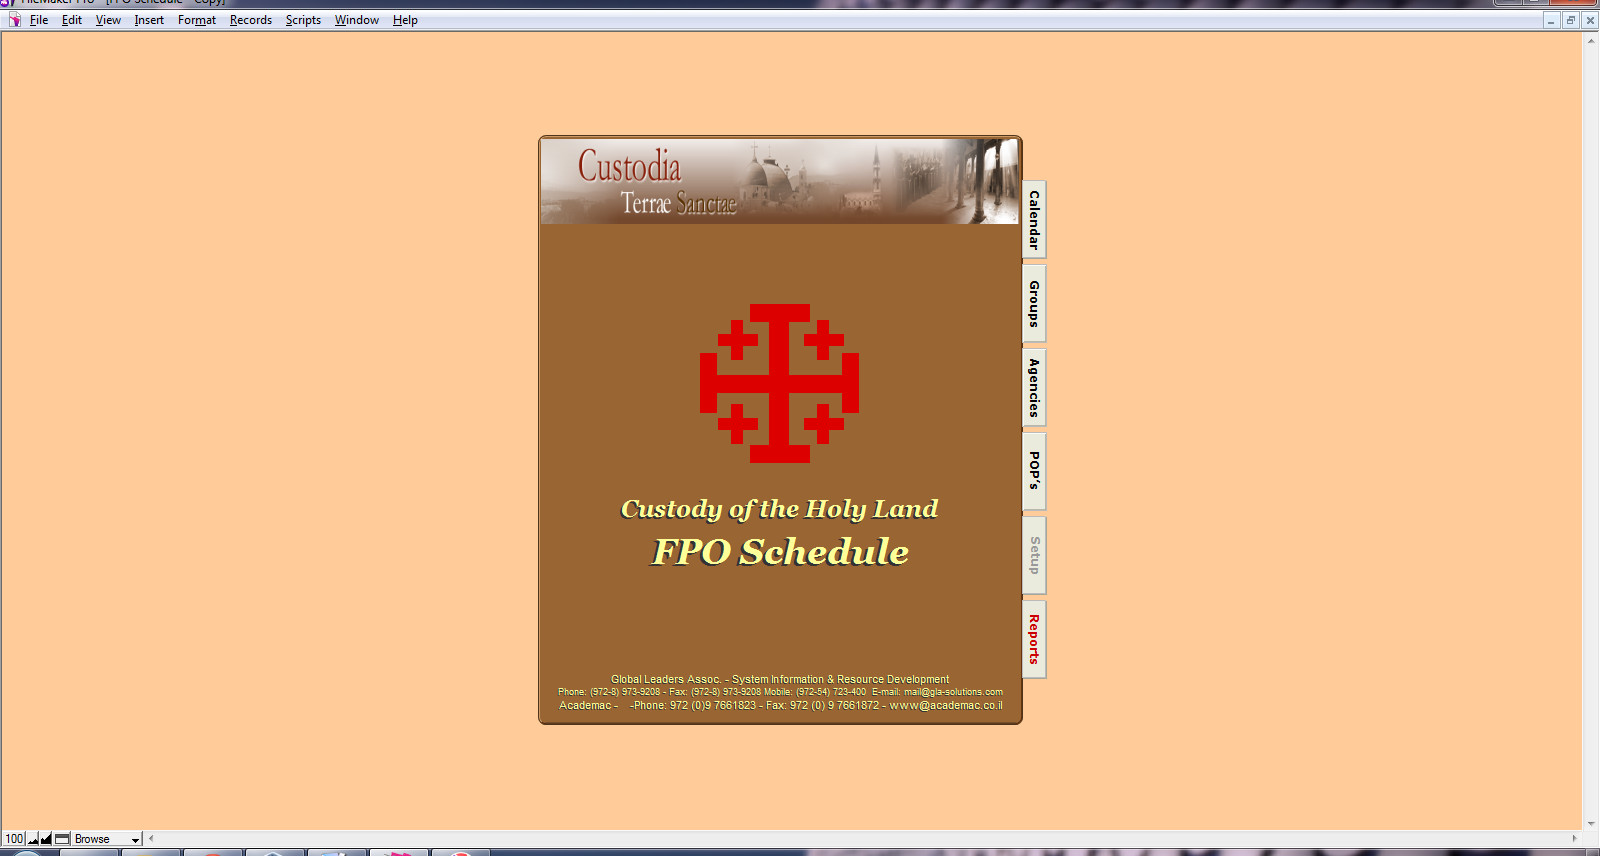
\includegraphics[width=.6\linewidth]{FPOSchedule1.jpg}
\end{frame}

\begin{frame}{Aktualna aplikacja CICTS}{tutuł innego obrazka}
   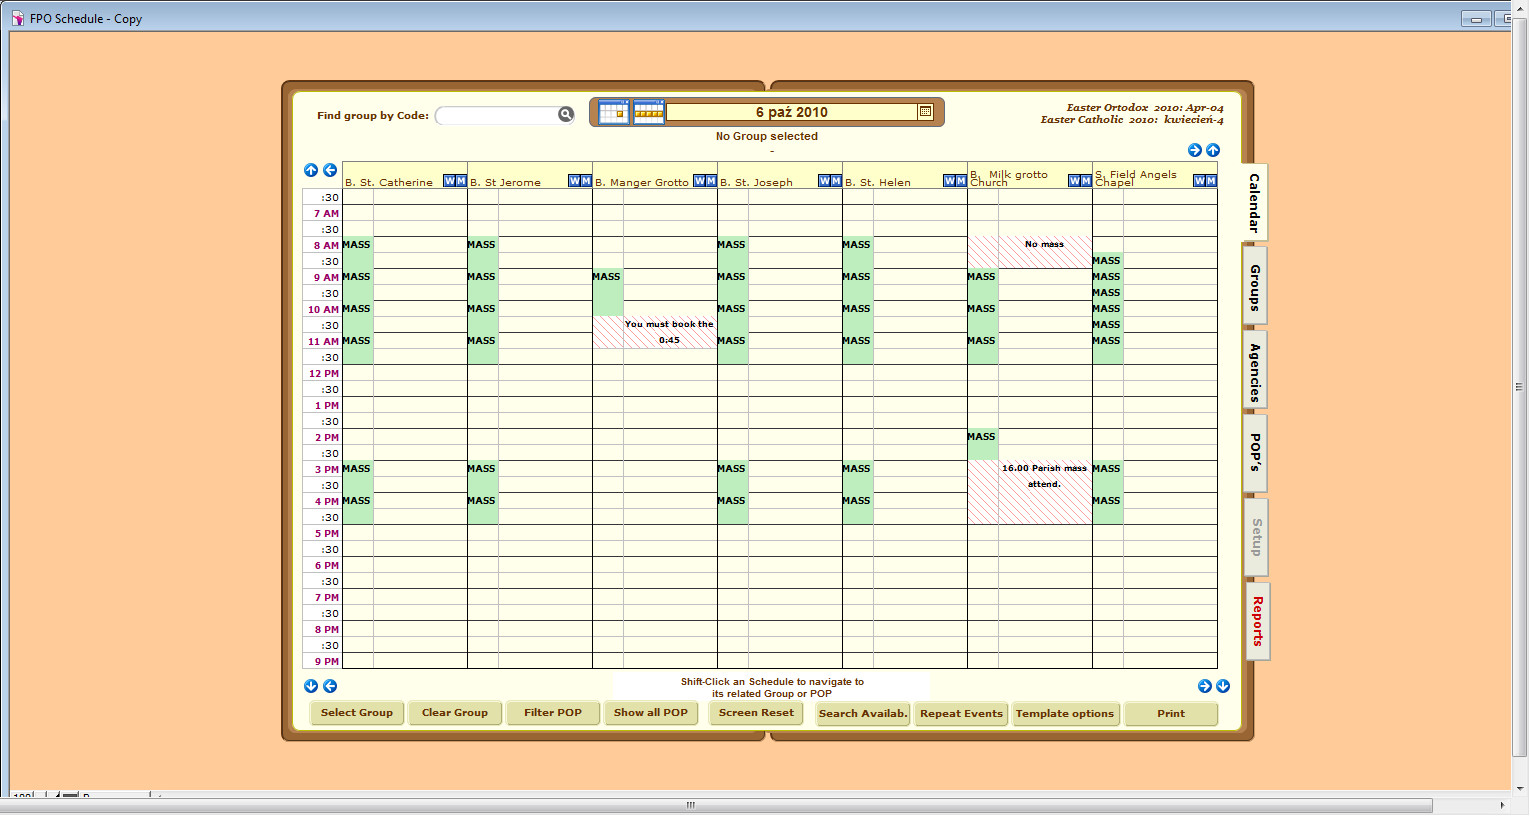
\includegraphics[width=.6\linewidth]{FPOSchedule2.jpg}
\end{frame}

\begin{frame}{Aktualna aplikacja CICTS}{tutuł kolejnego obrazka}
   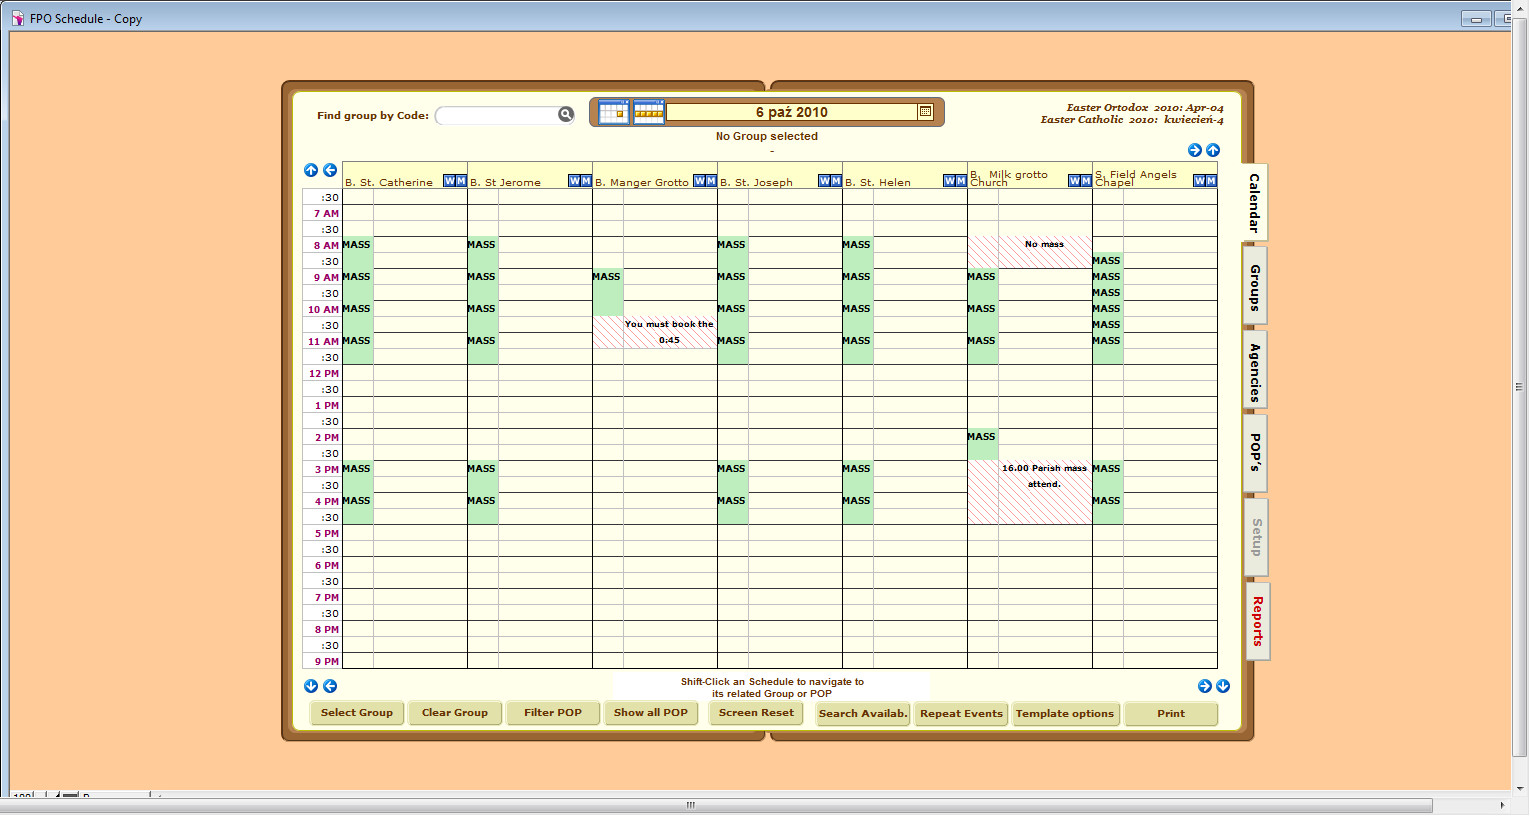
\includegraphics[width=.6\linewidth]{FPOSchedule2.jpg}
\end{frame}

\begin{frame}{Motywacja do modernizacji}
    \begin{block}{Wady technologiczne}
        \begin{itemize}
        \item bo tak
        \item bo w ogóle
        \end{itemize}
    \end{block}

    \begin{block}{Wady użytkowe}
        \begin{itemize}
        \item bo tak
        \item bo w ogóle
        \end{itemize}
    \end{block}
\end{frame}

\subsection{Aplikacja zmodernizowana}

\begin{frame}{Założenia modernizacyjne}
    \begin{block}{Technologie}
        \begin{itemize}
        \item bo tak
        \item bo w ogóle
        \end{itemize}
    \end{block}

    \begin{block}{Usprawnienia UX}
        \begin{itemize}
        \item bo tak
        \item bo w ogóle
        \end{itemize}
    \end{block}
\end{frame}

\section{Postęp prac}

\begin{frame}{Stan przygotowania pracy dyplomowej}
    \begin{itemize}
    \item opracowano plan pracy
    \item przygotowano szablon pracy (skład w \LaTeX)
    \item wersjonowane są kody źródłowe i treść pracy 
          {\footnotesize (repozytorium \textsl{gitosis@poligon.tomaszkowalski.info:at.git}) }
    \item wdrożone QA {\footnotesize (za pośrednictwem Redmine \textsl{http://poligon.tomaszkowalski.info/redmine/projets/at12}) }
    \item opracowano mock-up interfejsu z widget-em kalendarza
    \end{itemize}
\end{frame}

\end{document}
